%!TEX root = volumeFinal.tex 
\chapter{\label{chap:games}Jogos}
 
  Jogos eletrônicos são muito populares, principalmente pela grande quantidade de gêneros, existem jogos de ação, aventura, esportes, estrategia, entre outros. Hoje em dia, os jogos buscam que quem jogue consiga ficar imerso no dentro do jogo, sem conseguir identificar um padrão nos jogadores fictícios, pois se não o jogo deixa de ser tão interessante. Para que isso aconteça, a IA é associada a diversos jogos, e é comum pensar que quanto mais complexa a IA aplicada dentro do jogo mais difícil jogo irá ficar, mas isso nem sempre é verdade, nem sempre IA complicadas terão melhor desempenho do que as mais simples, uma boa IA dentro do jogo é feita a partir de determinar o comportamento certo para os algoritmo certos \cite{millington2009artificial}.
  
 \section{Jogos de estratégia em tempo real}
 
Jogos de estratégia em tempo real, também conhecido por \textit{real-time strategy games} (RTS), é um sub-gênero de jogos de estrategia, onde os jogadores precisam construir uma base com uma economia, ganhando recursos, construindo edificações, treinando unidades de ataques e tecnologias para elas, tudo isso com o objetivo de destruir uma ou mais bases inimigas \cite{ontanon2013survey, buro2012real}. 

Existem algumas diferenças entre jogos RTS e jogos de tabuleiro, como xadrez. Estas diferenças são \cite{ontanon2013survey}:

\begin{itemize}
	\item Movimentos simultâneos- jogadores realizam jogadas ao mesmo tempo;
	\item Tempo real- cada jogador deve realizar suas ações em um curto espaço de tempo;
	\item Parcialmente observável- na maioria dos jogos RTS, o jogador só consegue enxergar parte do ambiente;
	\item Não-determinístico- nem sempre uma ação realizada resulta  na saída esperada;
	\item Complexidade- O espaço de estados e o número de ações possíveis é muito grande.
\end{itemize} 


Pelo fato de existirem essas diferenças, não é possível traduzir automaticamente as técnicas padrões dos jogos de tabuleiro para jogos RTS sem algum tipo de abstração ou simplificação \cite{ontanon2013survey}.
 
\subsection{MicroRTS}  
 
Um exemplo deste gênero é o Starcraft\footnote{http://us.battle.net/sc2/pt/}. Uma simplificação do Starcraft foi feita por Santiago Ontañón \cite{ontanon2013combinatorial}, chamada de MicroRTS. O MicroRTS foi desenvolvido para fins acadêmicos, com o intuito de aplicar e desenvolver técnicas de IA e para servir como prova de conceito para as técnicas criadas.

\todo[inline]{como o jogo funciona?} 
O objetivo do jogo é destruir a base adversaria. Existem trabalhadores que podem coletar recursos e construir outros prédios. Os recursos são coletados dos minerais. Com os recursos é possível construir bases de ataque, onde são realizado o treinamento de unidades de ataque. Para conseguir realizar o objetivo de destruir a base adversaria é preciso ter unidades de ataque. O jogo oferece três destas unidades, são elas:
 
 \begin{itemize}
 	\item Heavy - Possui um alto poder de ataque, mas sua velocidade é lenta.
 	\item Light - Possui um baixo poder de ataque, mas sua velocidade é rápida.
 	\item Ranged - Possui um ataque de longa distancia. 
 \end{itemize} 
 
 A Figura~\ref{fig:microrts}\footnote{https://github.com/santiontanon/microrts} mostra uma tela do jogo que representa o que foi explicado e ainda é possível observar que o fator de ramificação pode ser muito alto dependendo do cenário do jogo.
 
 \begin{figure}[ht]
 	\centering
 	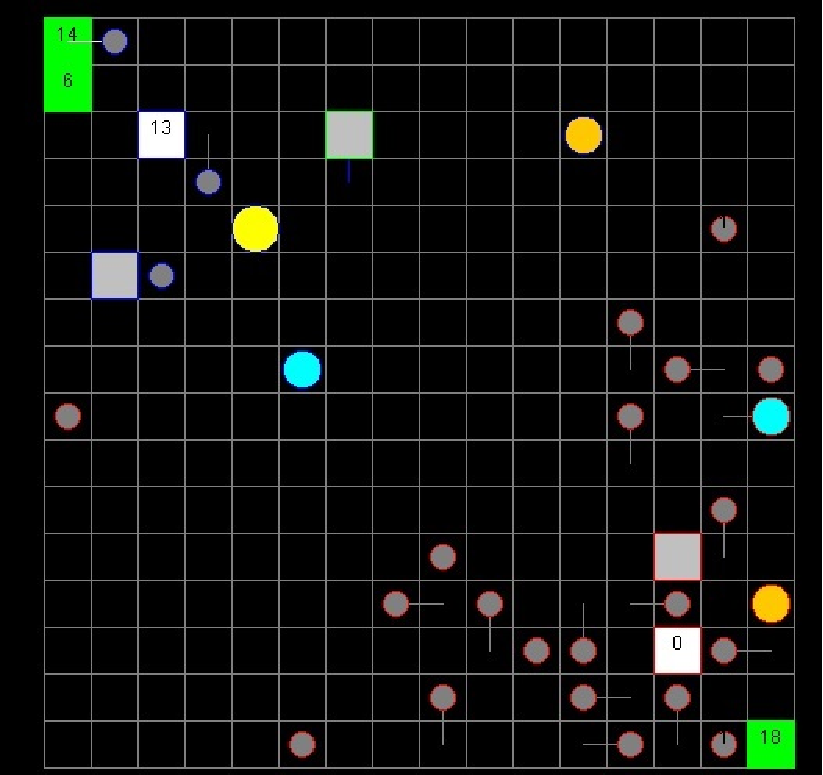
\includegraphics[width=0.5\textwidth]{fig/microrts.pdf}
 	\caption{Um exemplo de tela do MicroRTS}
 	\label{fig:microrts}
 \end{figure} 
 
\todo[inline]{abordagens já implementadas} 
No ambiente há algumas estrategias implementadas, cada estrategia possui variações dos algoritmos. Algumas das estrategias são:
 \begin{itemize}
 	\item Minimax Alpha-Beta Search Strategies - O que muda entre as técnicas é o jeito com que é feito a expansão do grafo.
 	\item Monte Carlo Search Strategies - Executa jogadas aleatórias para planejar e após utiliza uma heurística para determinar em qual caminho seguir.
 \end{itemize}
 
A plataforma já foi utilizada para aplicar técnica de IA. Por esse motivo a utilização dela se torna viável para a realização deste trabalho. 
 
 
 
 